\documentclass[journal=,manuscript=]{achemso}
\usepackage[version=3]{mhchem}
\usepackage{amsmath}
\newcommand*\mycommand[1]{\texttt{\emph{#1}}}


\keywords{3 to 6 keywords}

\title[]{}
\makeatletter
\ifxetex
  \usepackage[setpagesize=false, % page size defined by xetex
              unicode=false, % unicode breaks when used with xetex
              xetex]{hyperref}
\else
  \usepackage[unicode=true]{hyperref}
\fi
\hypersetup{breaklinks=true,
            bookmarks=true,
            pdfauthor={},
            pdftitle={An R Markdown template for report},
            colorlinks=true,
            urlcolor=blue,
            linkcolor=magenta,
            pdfborder={0 0 0}}
\urlstyle{same}  % don't use monospace font for urls
% Make links footnotes instead of hotlinks:
\renewcommand{\href}[2]{#2\footnote{\url{#1}}}


% pandoc header
\usepackage{color}
\usepackage{fancyvrb}
\newcommand{\VerbBar}{|}
\newcommand{\VERB}{\Verb[commandchars=\\\{\}]}
\DefineVerbatimEnvironment{Highlighting}{Verbatim}{commandchars=\\\{\}}
% Add ',fontsize=\small' for more characters per line
\usepackage{framed}
\definecolor{shadecolor}{RGB}{248,248,248}
\newenvironment{Shaded}{\begin{snugshade}}{\end{snugshade}}
\newcommand{\KeywordTok}[1]{\textcolor[rgb]{0.13,0.29,0.53}{\textbf{#1}}}
\newcommand{\DataTypeTok}[1]{\textcolor[rgb]{0.13,0.29,0.53}{#1}}
\newcommand{\DecValTok}[1]{\textcolor[rgb]{0.00,0.00,0.81}{#1}}
\newcommand{\BaseNTok}[1]{\textcolor[rgb]{0.00,0.00,0.81}{#1}}
\newcommand{\FloatTok}[1]{\textcolor[rgb]{0.00,0.00,0.81}{#1}}
\newcommand{\ConstantTok}[1]{\textcolor[rgb]{0.00,0.00,0.00}{#1}}
\newcommand{\CharTok}[1]{\textcolor[rgb]{0.31,0.60,0.02}{#1}}
\newcommand{\SpecialCharTok}[1]{\textcolor[rgb]{0.00,0.00,0.00}{#1}}
\newcommand{\StringTok}[1]{\textcolor[rgb]{0.31,0.60,0.02}{#1}}
\newcommand{\VerbatimStringTok}[1]{\textcolor[rgb]{0.31,0.60,0.02}{#1}}
\newcommand{\SpecialStringTok}[1]{\textcolor[rgb]{0.31,0.60,0.02}{#1}}
\newcommand{\ImportTok}[1]{#1}
\newcommand{\CommentTok}[1]{\textcolor[rgb]{0.56,0.35,0.01}{\textit{#1}}}
\newcommand{\DocumentationTok}[1]{\textcolor[rgb]{0.56,0.35,0.01}{\textbf{\textit{#1}}}}
\newcommand{\AnnotationTok}[1]{\textcolor[rgb]{0.56,0.35,0.01}{\textbf{\textit{#1}}}}
\newcommand{\CommentVarTok}[1]{\textcolor[rgb]{0.56,0.35,0.01}{\textbf{\textit{#1}}}}
\newcommand{\OtherTok}[1]{\textcolor[rgb]{0.56,0.35,0.01}{#1}}
\newcommand{\FunctionTok}[1]{\textcolor[rgb]{0.00,0.00,0.00}{#1}}
\newcommand{\VariableTok}[1]{\textcolor[rgb]{0.00,0.00,0.00}{#1}}
\newcommand{\ControlFlowTok}[1]{\textcolor[rgb]{0.13,0.29,0.53}{\textbf{#1}}}
\newcommand{\OperatorTok}[1]{\textcolor[rgb]{0.81,0.36,0.00}{\textbf{#1}}}
\newcommand{\BuiltInTok}[1]{#1}
\newcommand{\ExtensionTok}[1]{#1}
\newcommand{\PreprocessorTok}[1]{\textcolor[rgb]{0.56,0.35,0.01}{\textit{#1}}}
\newcommand{\AttributeTok}[1]{\textcolor[rgb]{0.77,0.63,0.00}{#1}}
\newcommand{\RegionMarkerTok}[1]{#1}
\newcommand{\InformationTok}[1]{\textcolor[rgb]{0.56,0.35,0.01}{\textbf{\textit{#1}}}}
\newcommand{\WarningTok}[1]{\textcolor[rgb]{0.56,0.35,0.01}{\textbf{\textit{#1}}}}
\newcommand{\AlertTok}[1]{\textcolor[rgb]{0.94,0.16,0.16}{#1}}
\newcommand{\ErrorTok}[1]{\textcolor[rgb]{0.64,0.00,0.00}{\textbf{#1}}}
\newcommand{\NormalTok}[1]{#1}

\usepackage{amsthm}
\newtheorem{theorem}{Theorem}[section]
\newtheorem{lemma}{Lemma}[section]
\newtheorem{corollary}{Corollary}[section]
\newtheorem{proposition}{Proposition}[section]
\newtheorem{conjecture}{Conjecture}[section]
\theoremstyle{definition}
\newtheorem{definition}{Definition}[section]
\theoremstyle{definition}
\newtheorem{example}{Example}[section]
\theoremstyle{definition}
\newtheorem{exercise}{Exercise}[section]
\theoremstyle{remark}
\newtheorem*{remark}{Remark}
\newtheorem*{solution}{Solution}
\begin{document}
\begin{abstract}
The text of your abstract. 200 or fewer words.
\end{abstract}
The header.tex file enable this template to show code correctly.

\hypertarget{preface}{%
\section{Preface}\label{preface}}

\hypertarget{markdown-elements}{%
\section{markdown elements}\label{markdown-elements}}

normal content:

Lorem ipsum dolor sit amet, consectetur adipisicing elit. Quisquam, nulla? Magni quia quo eaque porro consequatur molestias ratione hic sapiente possimus totam omnis accusantium illum voluptatem esse cumque assumenda quidem, facere officiis, exercitationem architecto, nam excepturi similique. Vitae, quod non. Sunt dignissimos, saepe quidem cum atque eum commodi illo autem eaque dolor, aut vel quod veniam neque, unde natus. Veritatis accusamus voluptates nihil animi? Cumque omnis blanditiis eveniet earum adipisci architecto eum laudantium velit quos exercitationem, consectetur natus. Voluptatibus, quibusdam est assumenda veniam accusantium voluptatem, sed perspiciatis ea iure saepe tenetur repudiandae nobis nemo accusamus et provident aut illum ipsa tempore eius architecto distinctio perferendis laudantium ratione. Itaque, voluptates! Praesentium incidunt eos animi laboriosam modi ullam ut totam voluptate sit necessitatibus repellendus numquam iure quibusdam ea facere ratione laborum, impedit dolorem tempora! Vero, ea deleniti voluptas quasi ducimus molestiae. Inventore autem corrupti dolorum itaque nesciunt, tenetur esse ratione tempore. Molestiae mollitia numquam ea, ex fugit rem inventore quasi libero in officiis eaque nesciunt natus reprehenderit eos a. Laborum exercitationem, explicabo non ab vitae optio minima eveniet sapiente et ad a vero sed distinctio fugit harum numquam qui atque assumenda illo. Illo omnis vitae hic nemo quaerat officiis laudantium dolore earum!

\textbf{bold}

\emph{italic}

quote

\begin{quote}
this is a block of quote
\end{quote}

\href{https://qiushi.rbind.io}{link}

code

\begin{Shaded}
\begin{Highlighting}[]
\KeywordTok{print}\NormalTok{(}\StringTok{"hello world"}\NormalTok{)}
\CommentTok{#> [1] "hello world"}
\end{Highlighting}
\end{Shaded}

table

\begin{Shaded}
\begin{Highlighting}[]
\NormalTok{knitr}\OperatorTok{::}\KeywordTok{kable}\NormalTok{(}\KeywordTok{head}\NormalTok{(iris))}
\end{Highlighting}
\end{Shaded}

\begin{tabular}{r|r|r|r|l}
\hline
Sepal.Length & Sepal.Width & Petal.Length & Petal.Width & Species\\
\hline
5.1 & 3.5 & 1.4 & 0.2 & setosa\\
\hline
4.9 & 3.0 & 1.4 & 0.2 & setosa\\
\hline
4.7 & 3.2 & 1.3 & 0.2 & setosa\\
\hline
4.6 & 3.1 & 1.5 & 0.2 & setosa\\
\hline
5.0 & 3.6 & 1.4 & 0.2 & setosa\\
\hline
5.4 & 3.9 & 1.7 & 0.4 & setosa\\
\hline
\end{tabular}

\hypertarget{cross-referencing-special-environment-footnotes}{%
\section{cross referencing, special environment, footnotes}\label{cross-referencing-special-environment-footnotes}}

cross reference for figure \ref{fig:mtcars}

\begin{Shaded}
\begin{Highlighting}[]
\KeywordTok{plot}\NormalTok{(mtcars[}\DecValTok{1}\OperatorTok{:}\DecValTok{2}\NormalTok{])}
\end{Highlighting}
\end{Shaded}

\begin{figure}

{\centering 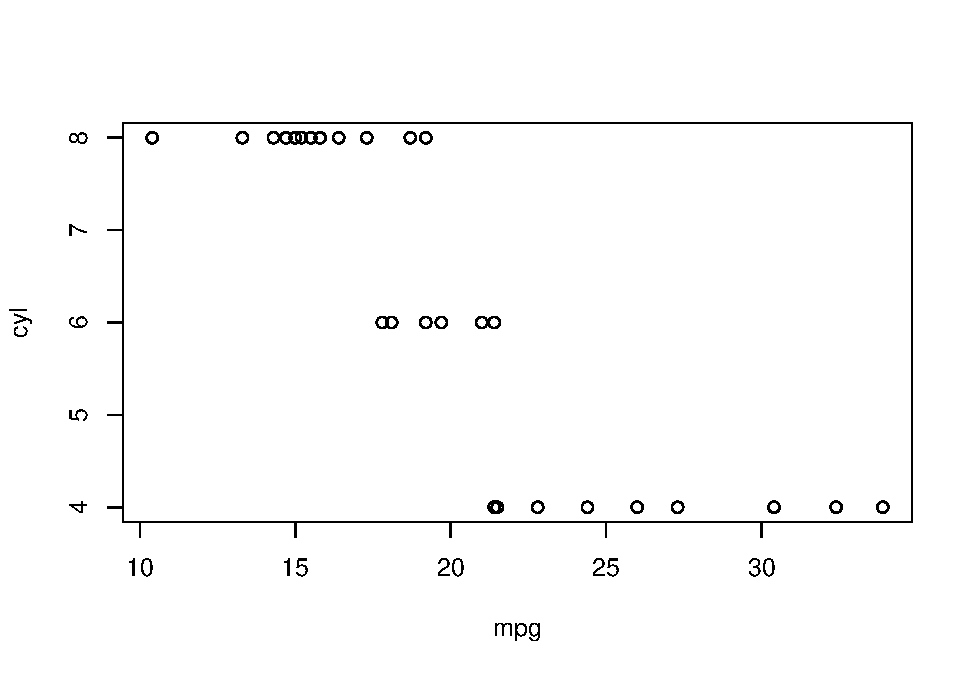
\includegraphics{acs_article_files/figure-latex/mtcars-1} 

}

\caption{this is a figrue}\label{fig:mtcars}
\end{figure}

cross reference for equation \eqref{eq:my-eq}

\begin{equation}
\label{eq:my-eq}
a^2 + b^2 = c^2
\end{equation}

Theorem \ref{thm:my-theorem} shows what I want to tell you.

\begin{theorem}[a fancy theorem of mine]
\protect\hypertarget{thm:my-theorem}{}{\label{thm:my-theorem} \iffalse (a fancy theorem of mine) \fi{} }In fact, what I want to tell you is that this theorem is meaningless.
\end{theorem}

This is a footnote\footnote{this is a footnote}

\hypertarget{introduction}{%
\section{Introduction}\label{introduction}}

table of contents

subtitles

This template demonstrates some of the basic latex you'll need to know to create a ASA article.

\section{Verifications}
\label{sec:verify}

This section will be just long enough to illustrate what a full page of
text looks like, for margins and spacing.

Campbell and Austin (\protect\hyperlink{ref-Campbell02}{2002}) Schubert et al. (\protect\hyperlink{ref-Schubert13}{2013}; Chi, Feltovich, and Glaser \protect\hyperlink{ref-Chi81}{1981})

\hypertarget{discussion}{%
\section{Discussion}\label{discussion}}

math environments

\[
a^2 + b^2 = c^2 
\]
cross referencing theorem \ref{thm:pyth}

\begin{theorem}[Pythagorean theorem]
\protect\hypertarget{thm:pyth}{}{\label{thm:pyth} \iffalse (Pythagorean theorem) \fi{} }For a right triangle, if \(c\) denotes the length of the hypotenuse
and \(a\) and \(b\) denote the lengths of the other two sides, we have

\[a^2 + b^2 = c^2\]
\end{theorem}

\hypertarget{conclusion}{%
\section{Conclusion}\label{conclusion}}

cross referencing figures \ref{fig:diamond-plot}

\begin{Shaded}
\begin{Highlighting}[]
\KeywordTok{library}\NormalTok{(dplyr)}
\KeywordTok{library}\NormalTok{(ggplot2)}

\NormalTok{diamonds }\OperatorTok\StringTok{ }
\StringTok{  }\KeywordTok{slice_sample}\NormalTok{(}\DataTypeTok{n =} \DecValTok{500}\NormalTok{) }\OperatorTok
\StringTok{  }\KeywordTok{ggplot}\NormalTok{() }\OperatorTok{+}\StringTok{ }
\StringTok{  }\KeywordTok{geom_point}\NormalTok{(}\KeywordTok{aes}\NormalTok{(carat, price, }\DataTypeTok{color =}\NormalTok{ cut)) }\OperatorTok{+}\StringTok{ }
\StringTok{  }\KeywordTok{theme_minimal}\NormalTok{()}
\end{Highlighting}
\end{Shaded}

\begin{figure}

{\centering 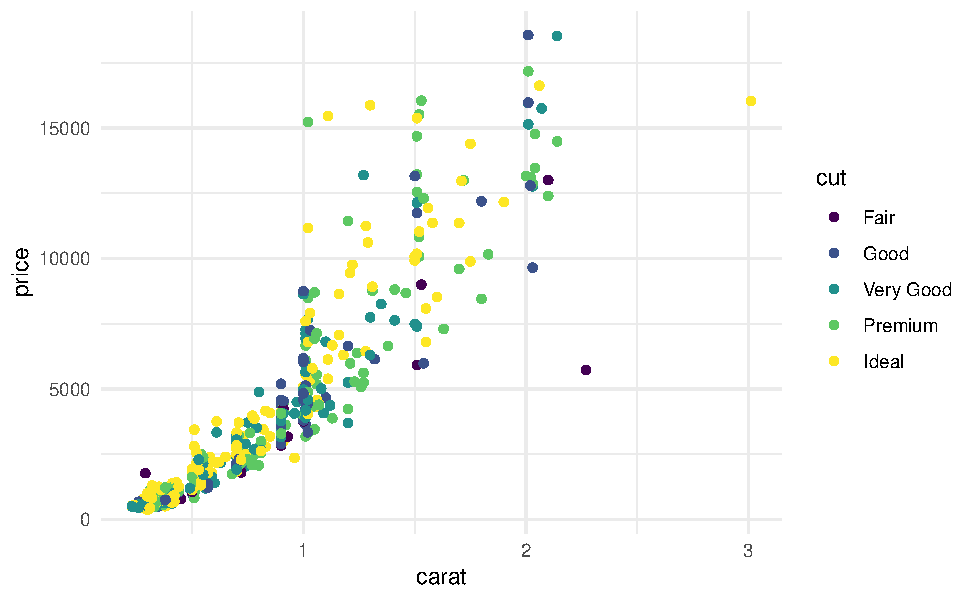
\includegraphics{acs_article_files/figure-latex/diamond-plot-1} 

}

\caption{this is a figure}\label{fig:diamond-plot}
\end{figure}

cross referencing tables \ref{tab:iris}

\begin{table}

\caption{\label{tab:iris}my table}
\centering
\begin{tabular}[t]{r|r|r|r|l}
\hline
Sepal.Length & Sepal.Width & Petal.Length & Petal.Width & Species\\
\hline
5.1 & 3.5 & 1.4 & 0.2 & setosa\\
\hline
4.9 & 3.0 & 1.4 & 0.2 & setosa\\
\hline
4.7 & 3.2 & 1.3 & 0.2 & setosa\\
\hline
4.6 & 3.1 & 1.5 & 0.2 & setosa\\
\hline
5.0 & 3.6 & 1.4 & 0.2 & setosa\\
\hline
5.4 & 3.9 & 1.7 & 0.4 & setosa\\
\hline
\end{tabular}
\end{table}

The quick brown fox jumped over the lazy dog.
The quick brown fox jumped over the lazy dog.
The quick brown fox jumped over the lazy dog.
The quick brown fox jumped over the lazy dog.
\textbf{With this spacing we have 30 lines per page.}

The quick brown fox jumped over the lazy dog.
The quick brown fox jumped over the lazy dog.
The quick brown fox jumped over the lazy dog.
The quick brown fox jumped over the lazy dog.
The quick brown fox jumped over the lazy dog.

The quick brown fox jumped over the lazy dog.
The quick brown fox jumped over the lazy dog.
The quick brown fox jumped over the lazy dog.
The quick brown fox jumped over the lazy dog.
The quick brown fox jumped over the lazy dog.
The quick brown fox jumped over the lazy dog.
The quick brown fox jumped over the lazy dog.
The quick brown fox jumped over the lazy dog.
The quick brown fox jumped over the lazy dog.
The quick brown fox jumped over the lazy dog.

The quick brown fox jumped over the lazy dog.
The quick brown fox jumped over the lazy dog.
The quick brown fox jumped over the lazy dog.
The quick brown fox jumped over the lazy dog.
The quick brown fox jumped over the lazy dog.
The quick brown fox jumped over the lazy dog.
The quick brown fox jumped over the lazy dog.
The quick brown fox jumped over the lazy dog.
The quick brown fox jumped over the lazy dog.
The quick brown fox jumped over the lazy dog.

The quick brown fox jumped over the lazy dog.
The quick brown fox jumped over the lazy dog.
The quick brown fox jumped over the lazy dog.
The quick brown fox jumped over the lazy dog.
The quick brown fox jumped over the lazy dog.
The quick brown fox jumped over the lazy dog.
The quick brown fox jumped over the lazy dog.
The quick brown fox jumped over the lazy dog.
The quick brown fox jumped over the lazy dog.
The quick brown fox jumped over the lazy dog.

The quick brown fox jumped over the lazy dog.
The quick brown fox jumped over the lazy dog.
The quick brown fox jumped over the lazy dog.
The quick brown fox jumped over the lazy dog.
The quick brown fox jumped over the lazy dog.
The quick brown fox jumped over the lazy dog.
The quick brown fox jumped over the lazy dog.
The quick brown fox jumped over the lazy dog.
The quick brown fox jumped over the lazy dog.
The quick brown fox jumped over the lazy dog.

The quick brown fox jumped over the lazy dog.
The quick brown fox jumped over the lazy dog.
The quick brown fox jumped over the lazy dog.
The quick brown fox jumped over the lazy dog.
The quick brown fox jumped over the lazy dog.
The quick brown fox jumped over the lazy dog.
The quick brown fox jumped over the lazy dog.
The quick brown fox jumped over the lazy dog.
The quick brown fox jumped over the lazy dog.
The quick brown fox jumped over the lazy dog.

The quick brown fox jumped over the lazy dog.
The quick brown fox jumped over the lazy dog.
The quick brown fox jumped over the lazy dog.
The quick brown fox jumped over the lazy dog.
The quick brown fox jumped over the lazy dog.
The quick brown fox jumped over the lazy dog.
The quick brown fox jumped over the lazy dog.
The quick brown fox jumped over the lazy dog.
The quick brown fox jumped over the lazy dog.
The quick brown fox jumped over the lazy dog.

The quick brown fox jumped over the lazy dog.
The quick brown fox jumped over the lazy dog.
The quick brown fox jumped over the lazy dog.
The quick brown fox jumped over the lazy dog.
The quick brown fox jumped over the lazy dog.
The quick brown fox jumped over the lazy dog.
The quick brown fox jumped over the lazy dog.
The quick brown fox jumped over the lazy dog.
The quick brown fox jumped over the lazy dog.
The quick brown fox jumped over the lazy dog.

The quick brown fox jumped over the lazy dog.
The quick brown fox jumped over the lazy dog.
The quick brown fox jumped over the lazy dog.
The quick brown fox jumped over the lazy dog.
The quick brown fox jumped over the lazy dog.
The quick brown fox jumped over the lazy dog.
The quick brown fox jumped over the lazy dog.
The quick brown fox jumped over the lazy dog.
The quick brown fox jumped over the lazy dog.
The quick brown fox jumped over the lazy dog.

The quick brown fox jumped over the lazy dog.
The quick brown fox jumped over the lazy dog.
The quick brown fox jumped over the lazy dog.
The quick brown fox jumped over the lazy dog.
The quick brown fox jumped over the lazy dog.
The quick brown fox jumped over the lazy dog.
The quick brown fox jumped over the lazy dog.
The quick brown fox jumped over the lazy dog.
The quick brown fox jumped over the lazy dog.
The quick brown fox jumped over the lazy dog.

The quick brown fox jumped over the lazy dog.
The quick brown fox jumped over the lazy dog.
The quick brown fox jumped over the lazy dog.
The quick brown fox jumped over the lazy dog.

\hypertarget{references}{%
\section*{References}\label{references}}
\addcontentsline{toc}{section}{References}

\hypertarget{refs}{}
\leavevmode\hypertarget{ref-Campbell02}{}%
Campbell, Jamie I. D., and Shauna Austin. 2002. ``Effects of Response Time Deadlines on Adults' Strategy Choices for Simple Addition.'' \emph{Memory \& Cognition} 30 (6): 988--94.

\leavevmode\hypertarget{ref-Chi81}{}%
Chi, Michelene T. H., Paul J. Feltovich, and Robert Glaser. 1981. ``Categorization and Representation of Physics Problems by Experts and Novices.'' \emph{Cognitive Science} 5 (2): 121--52.

\leavevmode\hypertarget{ref-Schubert13}{}%
Schubert, Christiane C, T Kent Denmark, Beth Crandall, Anna Grome, and James Pappas. 2013. ``Characterizing Novice-Expert Differences in Macrocognition: An Exploratory Study of Cognitive Work in the Emergency Department.'' \emph{Annals of Emergency Medicine} 61 (1): 96--109.
\end{document}
